\section{UI設計}
本システムはWebブラウザから利用する。
画面は利用者の役割に応じて、主催者向け、競技者向け、観戦者向け
に分ける。
主催者向け画面では、大会情報や競技者情報、試合情報の登録・管理を行い、
競技者向け画面では参加大会や自身の試合情報を確認する。
観戦者向け画面では、大会全体の進行状況や注目する競技者の情報を確認できる。

\begin{table}[H]
    \centering
    \caption{画面一覧}
    \label{tab:screen_list}
    \begin{tabularx}{\linewidth}{|l|l|l|X|}
        \hline
        \rowcolor{tableblue}
        \multicolumn{1}{|c|}{画面ID} & \multicolumn{1}{c|}{画面名} & \multicolumn{1}{c|}{利用者} & \multicolumn{1}{c|}{主な表示・操作} \\ \hline
        S-01 & ログイン画面 & 主催者・競技者・観戦者 & ログイン情報入力、認証、アカウント登録画面への遷移 \\ \hline
        S-02 & 大会一覧・検索画面 & 全利用者 & 大会一覧、検索条件、開催状況の絞り込み \\ \hline
        S-03 & 大会詳細画面 & 全利用者 & 大会概要、参加条件、進行状況、配信URL、参加登録への遷移 \\ \hline
        S-04 & 競技者登録画面 & 競技者 & 氏名、プレイヤー名、メールアドレス等の入力 \\ \hline
        S-05 & 競技者マイページ & 競技者 & 参加大会、参加登録状態、受付状態、対戦相手、試合予定、試合結果の確認 \\ \hline
        S-06 & 主催者ダッシュボード & 主催者 & 管理対象大会、参加登録者数、受付済み人数、未受付人数、進行中の試合状況の確認 \\ \hline
        S-07 & 大会作成・編集画面 & 主催者 & 大会情報、参加条件、大会形式、配信URLの登録・編集 \\ \hline
        S-08 & 競技者管理画面 & 主催者 & 競技者一覧、検索、受付済み/未受付の更新 \\ \hline
        S-09 & トーナメント・試合管理画面 & 主催者 & 組み合わせ作成、試合一覧、結果登録・確認・修正 \\ \hline
        S-10 & 大会観戦画面 & 観戦者 & トーナメント表、試合状況、試合結果、配信URL、お気に入り選手の情報の確認 \\ \hline
        S-11 & 選手詳細・追跡画面 & 観戦者 & 選手の現在・次回試合、選手成績、対戦履歴、お気に入り登録 \\ \hline
    \end{tabularx}
\end{table}

\subsection{画面レイアウト}
以下は外部設計段階での画面構成を示す。
具体的な色、フォント、ボタン寸法、スマートフォンでの細かな配置は
画面デザイン工程で確定する。

\subsubsection{ログイン画面（S-01）}
\begin{table}[H]
    \centering
    \caption{ログイン画面のレイアウト構成}
    \label{tab:ui_s01}
    \begin{tabularx}{0.8\linewidth}{|l|X|}
        \hline
        \rowcolor{tableblue}
        \multicolumn{1}{|c|}{領域} & \multicolumn{1}{c|}{表示・入力項目} \\ \hline
        ヘッダー & システム名「Play Line」 \\ \hline
        ログイン入力 & メールアドレス、パスワード \\ \hline
        操作 & ログインボタン、アカウント登録画面へのリンク、パスワード再設定へのリンク \\ \hline
        メッセージ & 入力誤り、認証失敗等のメッセージ \\ \hline
    \end{tabularx}
\end{table}

\begin{figure}[H]
    \centering
    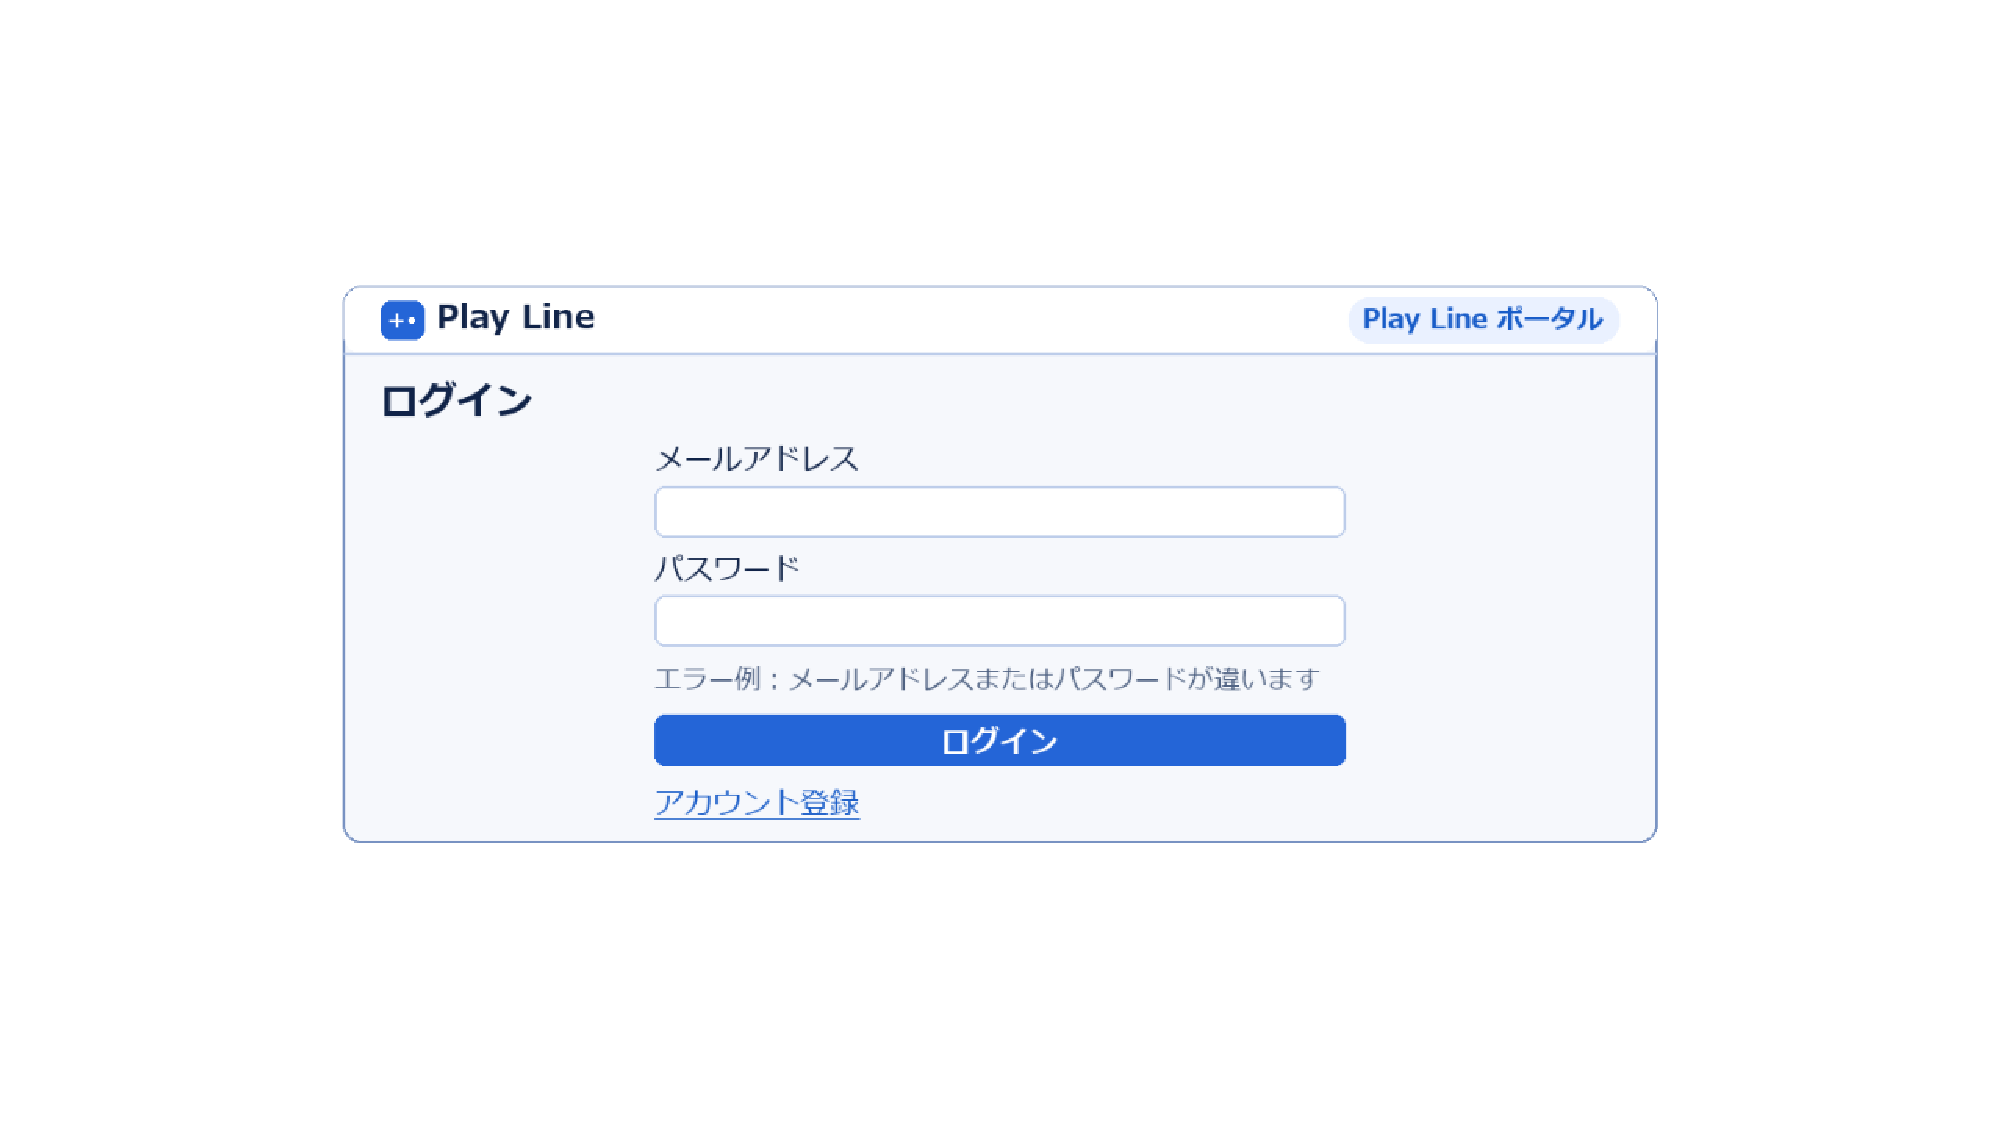
\includegraphics[width=\linewidth]{figures/04/s01_login.pdf}
    \caption{ログイン画面 UIイメージ}
    \label{fig:ui_s01}
\end{figure}

\subsubsection{大会一覧・検索画面（S-02）}
\begin{table}[H]
    \centering
    \caption{大会一覧・検索画面のレイアウト構成}
    \label{tab:ui_s02}
    \begin{tabularx}{0.8\linewidth}{|l|X|}
        \hline
        \rowcolor{tableblue}
        \multicolumn{1}{|c|}{領域} & \multicolumn{1}{c|}{表示・入力項目} \\ \hline
        検索条件 & 大会名、対象ゲーム、開催日、開催状況 \\ \hline
        大会一覧 & 大会名、開催日時、対象ゲーム、参加人数、受付状況 \\ \hline
        操作 & 検索、条件クリア、大会詳細へのリンク \\ \hline
    \end{tabularx}
\end{table}

\begin{figure}[H]
    \centering
    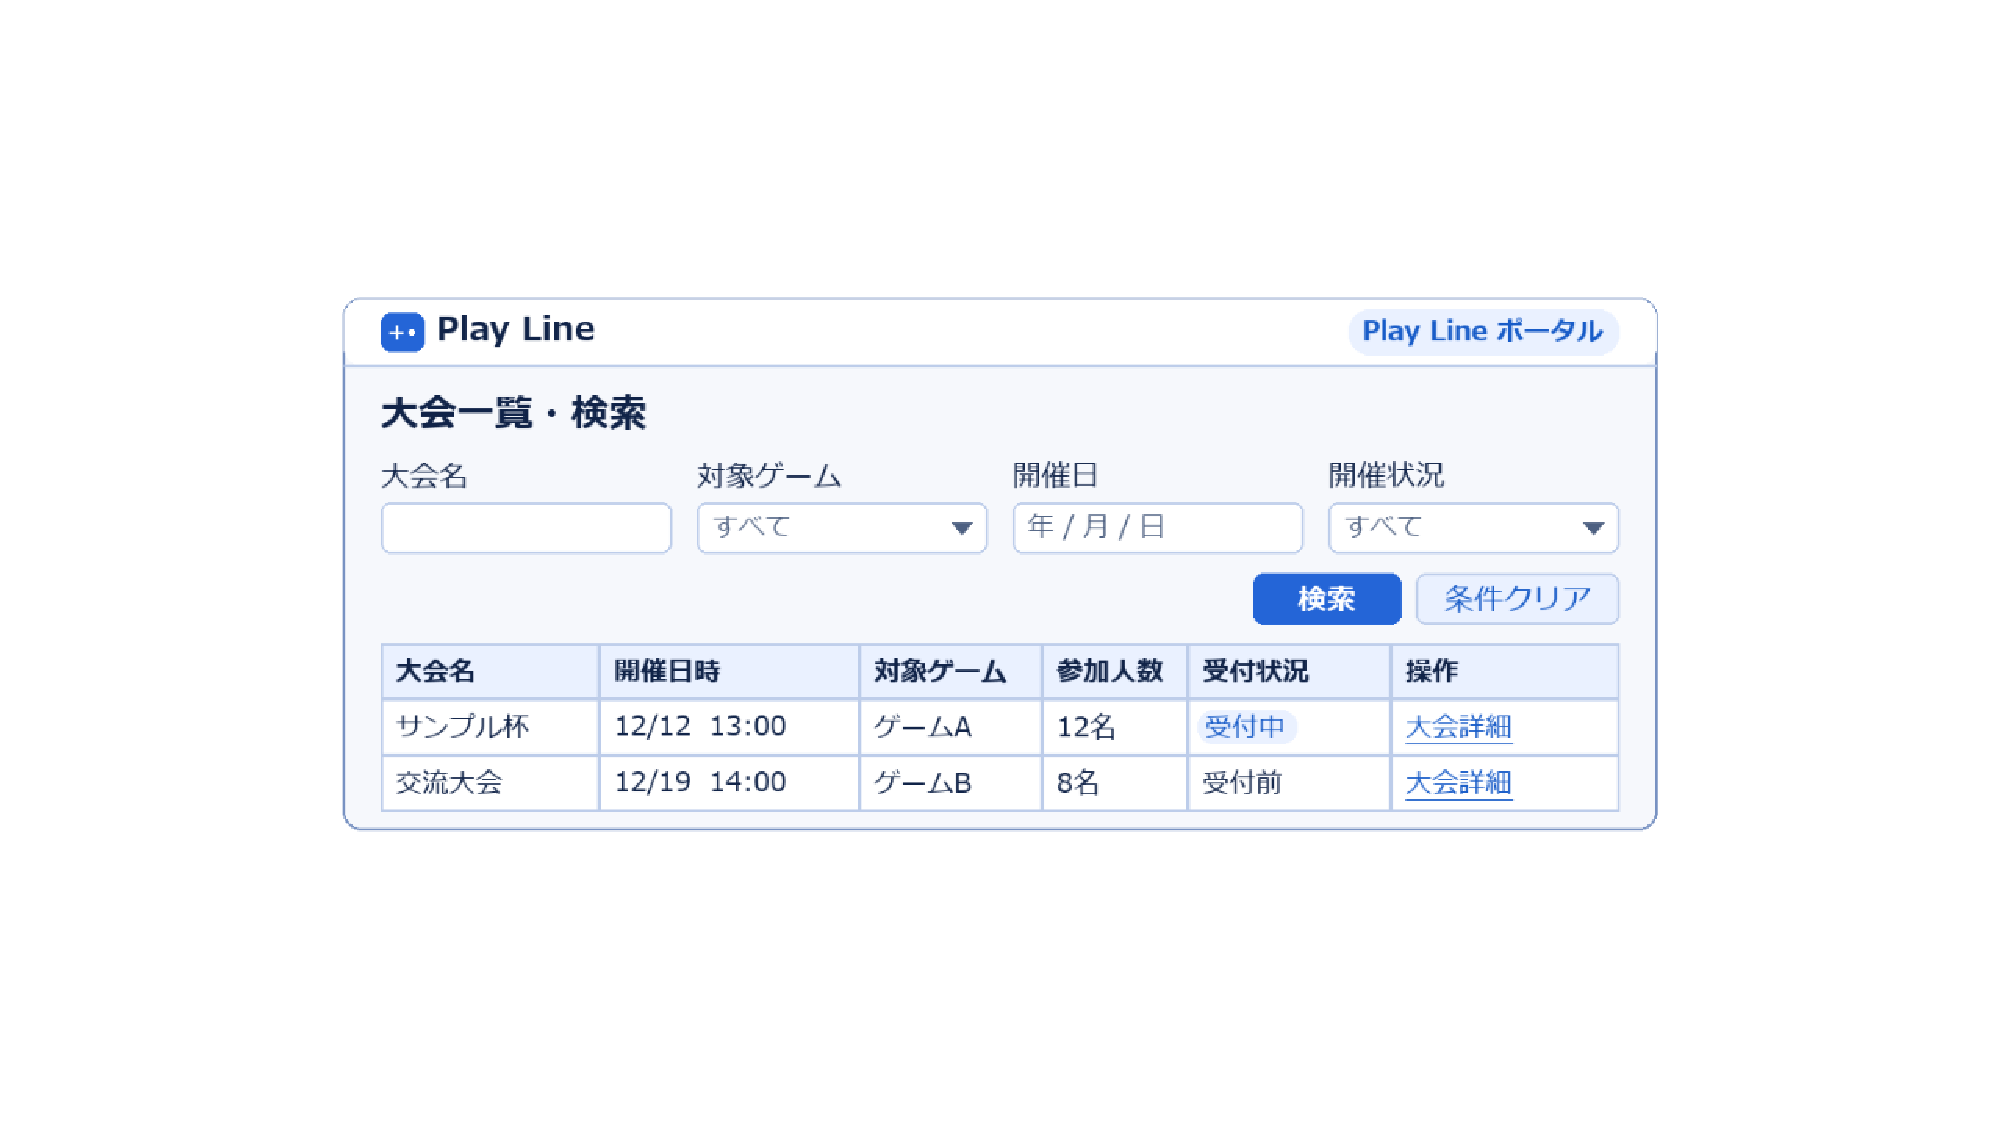
\includegraphics[width=\linewidth]{figures/04/s02_search.pdf}
    \caption{大会一覧・検索画面 UIイメージ}
    \label{fig:ui_s02}
\end{figure}

\subsubsection{大会詳細画面（S-03）}
\begin{table}[H]
    \centering
    \caption{大会詳細画面のレイアウト構成}
    \label{tab:ui_s03}
    \begin{tabularx}{0.8\linewidth}{|l|X|}
        \hline
        \rowcolor{tableblue}
        \multicolumn{1}{|c|}{領域} & \multicolumn{1}{c|}{表示・入力項目} \\ \hline
        大会概要 & 大会名、対象ゲーム、開催日時、開催場所、参加条件、大会形式 \\ \hline
        大会状況 & 参加登録状況、参加人数、開催状況 \\ \hline
        試合情報 & トーナメント表、試合一覧、結果、進行状況 \\ \hline
        配信情報 & 主催者が登録したライブ配信URL \\ \hline
        操作 & 参加登録、トーナメント・試合詳細の表示 \\ \hline
    \end{tabularx}
\end{table}

\begin{figure}[H]
    \centering
    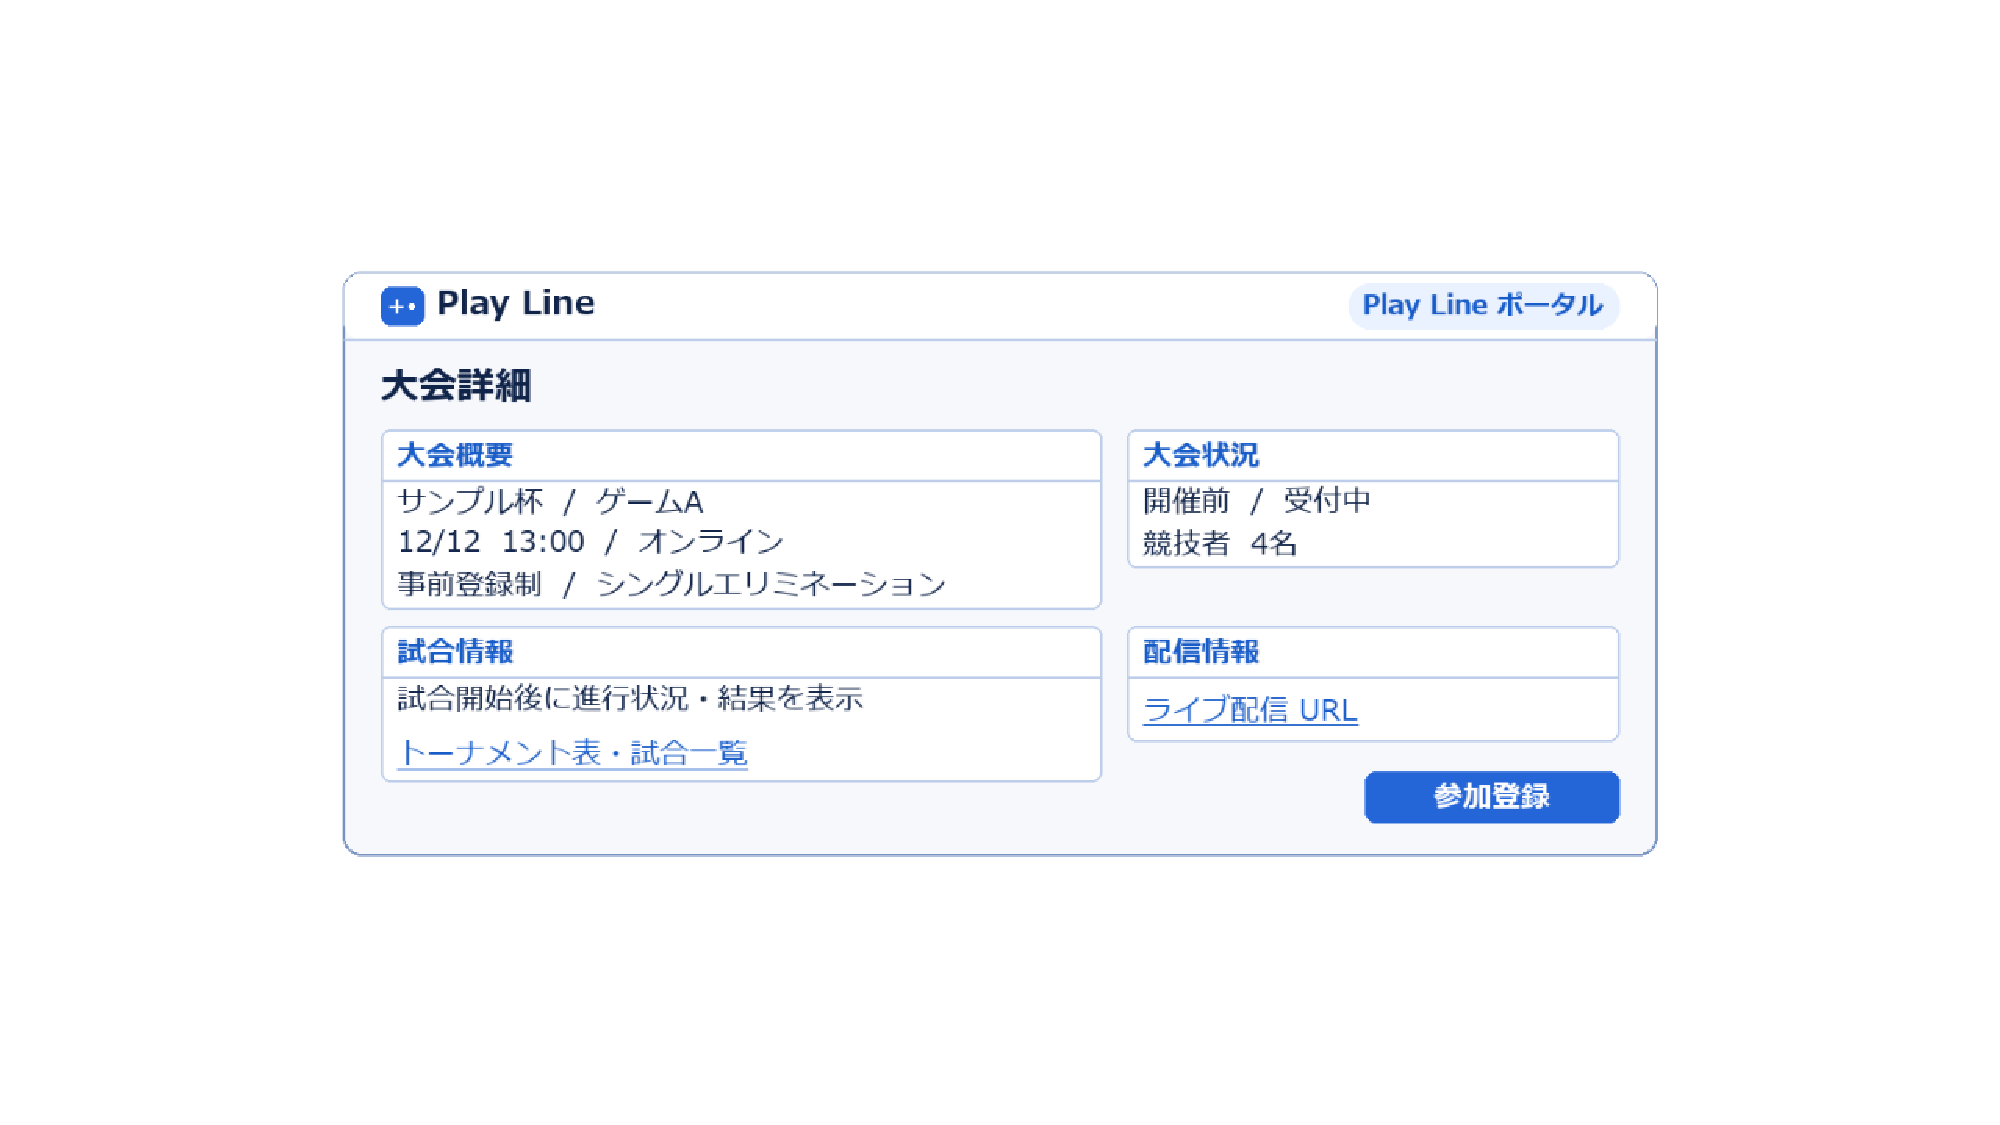
\includegraphics[width=\linewidth]{figures/04/s03_detail.pdf}
    \caption{大会詳細画面 UIイメージ}
    \label{fig:ui_s03}
\end{figure}

\subsubsection{競技者登録画面（S-04）}
\begin{table}[H]
    \centering
    \caption{競技者登録画面のレイアウト構成}
    \label{tab:ui_s04}
    \begin{tabularx}{0.8\linewidth}{|l|X|}
        \hline
        \rowcolor{tableblue}
        \multicolumn{1}{|c|}{領域} & \multicolumn{1}{c|}{表示・入力項目} \\ \hline
        入力項目 & 氏名、プレイヤー名、メールアドレス、パスワード等 \\ \hline
        確認 & 必須項目、入力形式、既存情報との重複 \\ \hline
        操作 & 登録、入力内容の修正 \\ \hline
        結果表示 & 登録完了またはエラーメッセージ \\ \hline
    \end{tabularx}
\end{table}

\begin{figure}[H]
    \centering
    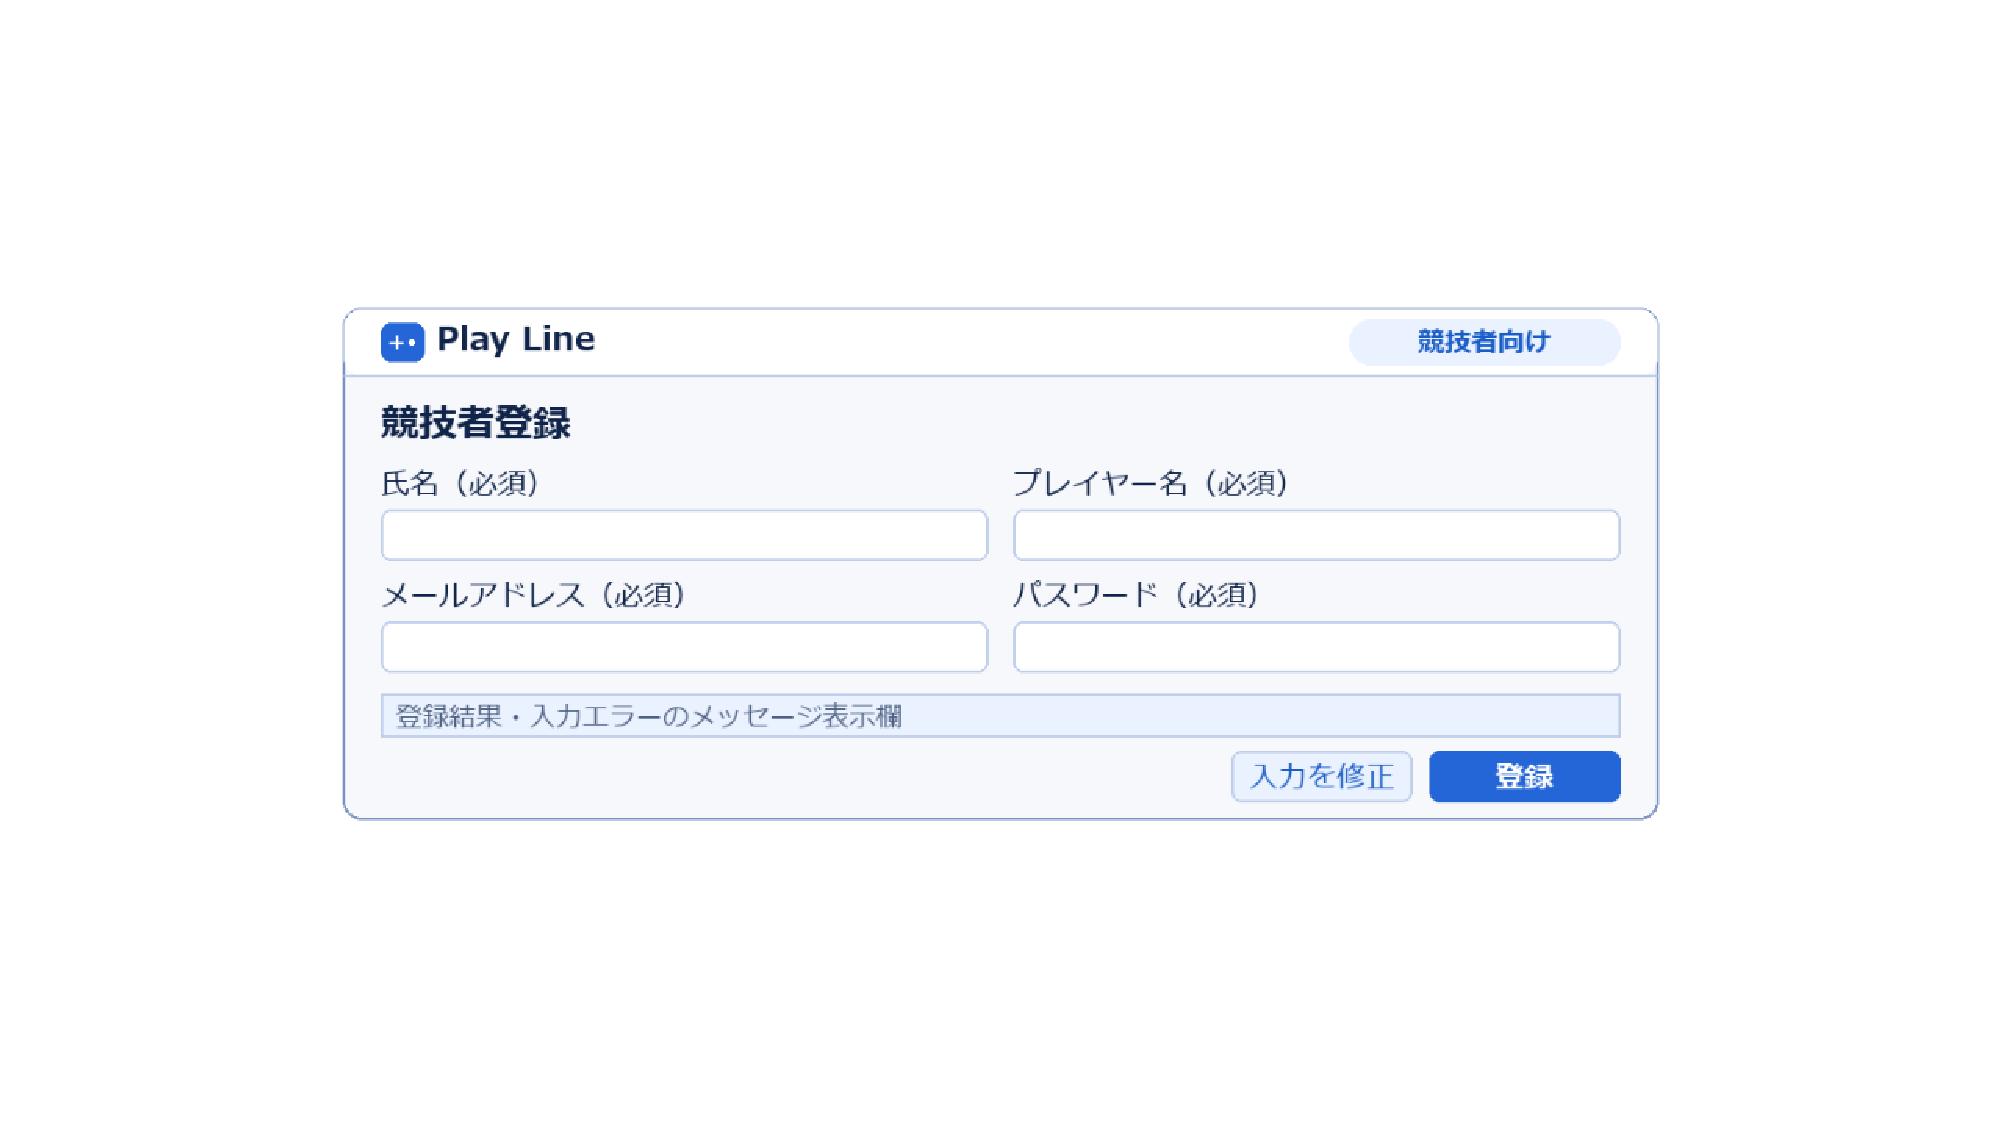
\includegraphics[width=\linewidth]{figures/04/s04_register.pdf}
    \caption{競技者登録画面 UIイメージ}
    \label{fig:ui_s04_img}
\end{figure}

\subsubsection{競技者マイページ（S-05）}
\begin{table}[H]
    \centering
    \caption{競技者マイページのレイアウト構成}
    \label{tab:ui_s05}
    \begin{tabularx}{0.8\linewidth}{|l|X|}
        \hline
        \rowcolor{tableblue}
        \multicolumn{1}{|c|}{領域} & \multicolumn{1}{c|}{表示・入力項目} \\ \hline
        参加大会 & 参加登録した大会、登録状態、受付状態 \\ \hline
        試合情報 & 試合予定、対戦相手、試合番号、試合状態 \\ \hline
        結果 & 自分の試合結果、トーナメント表における現在の位置 \\ \hline
        操作 & 試合結果の入力・確認（対象試合の場合） \\ \hline
    \end{tabularx}
\end{table}

\begin{figure}[H]
    \centering
    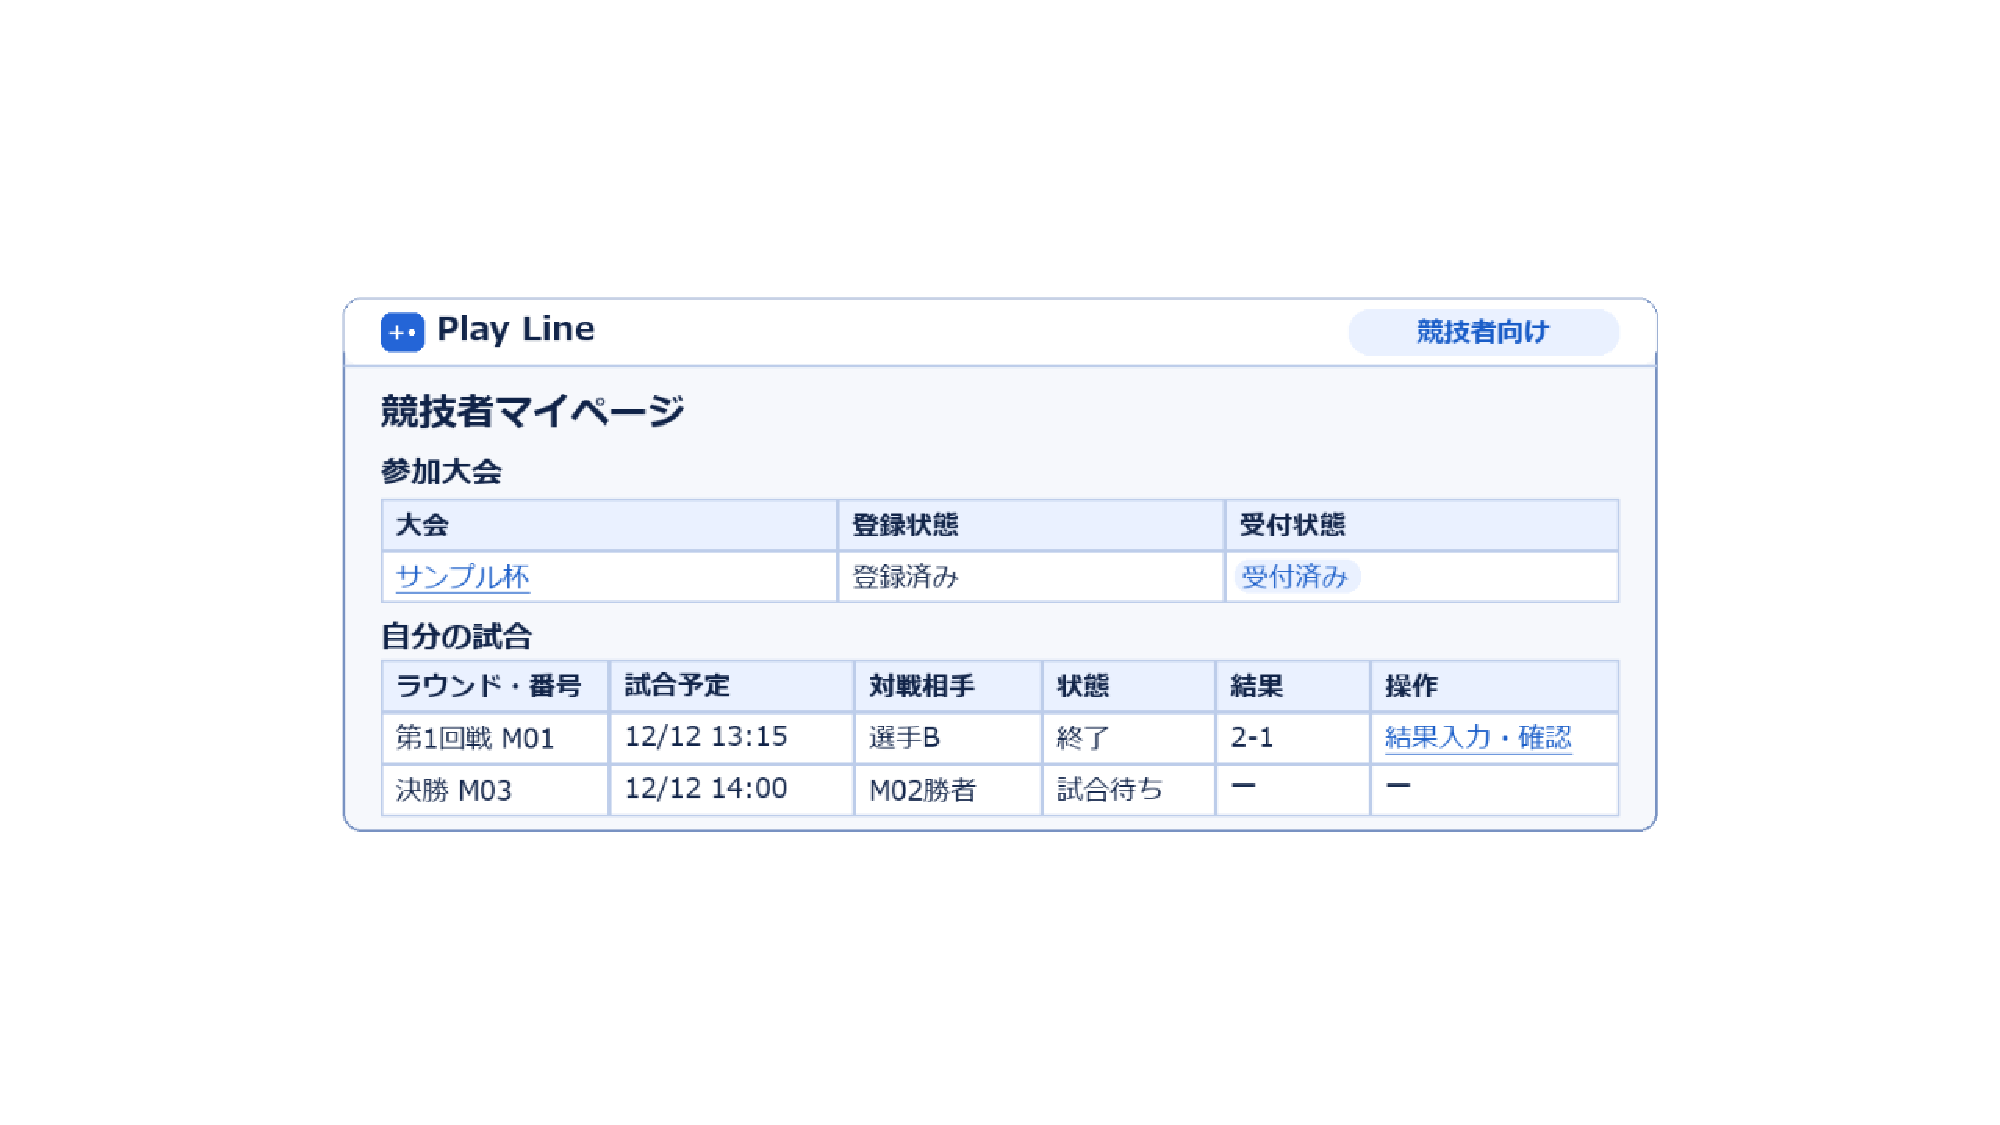
\includegraphics[width=\linewidth]{figures/04/s05_mypage.pdf}
    \caption{競技者マイページ UIイメージ}
    \label{fig:ui_s05_img}
\end{figure}

\subsubsection{主催者ダッシュボード画面（S-06）}
\begin{table}[H]
    \centering
    \caption{主催者ダッシュボード画面のレイアウト構成}
    \label{tab:ui_s06}
    \begin{tabularx}{0.8\linewidth}{|l|X|}
        \hline
        \rowcolor{tableblue}
        \multicolumn{1}{|c|}{領域} & \multicolumn{1}{c|}{表示・入力項目} \\ \hline
        大会概要 & 主催者が管理する大会の一覧、開催状況 \\ \hline
        運営状況 & 参加登録者数、受付済み人数、未受付人数、試合の進行状況 \\ \hline
        操作 & 大会作成、参加者管理、試合管理への遷移 \\ \hline
    \end{tabularx}
\end{table}

\begin{figure}[H]
    \centering
    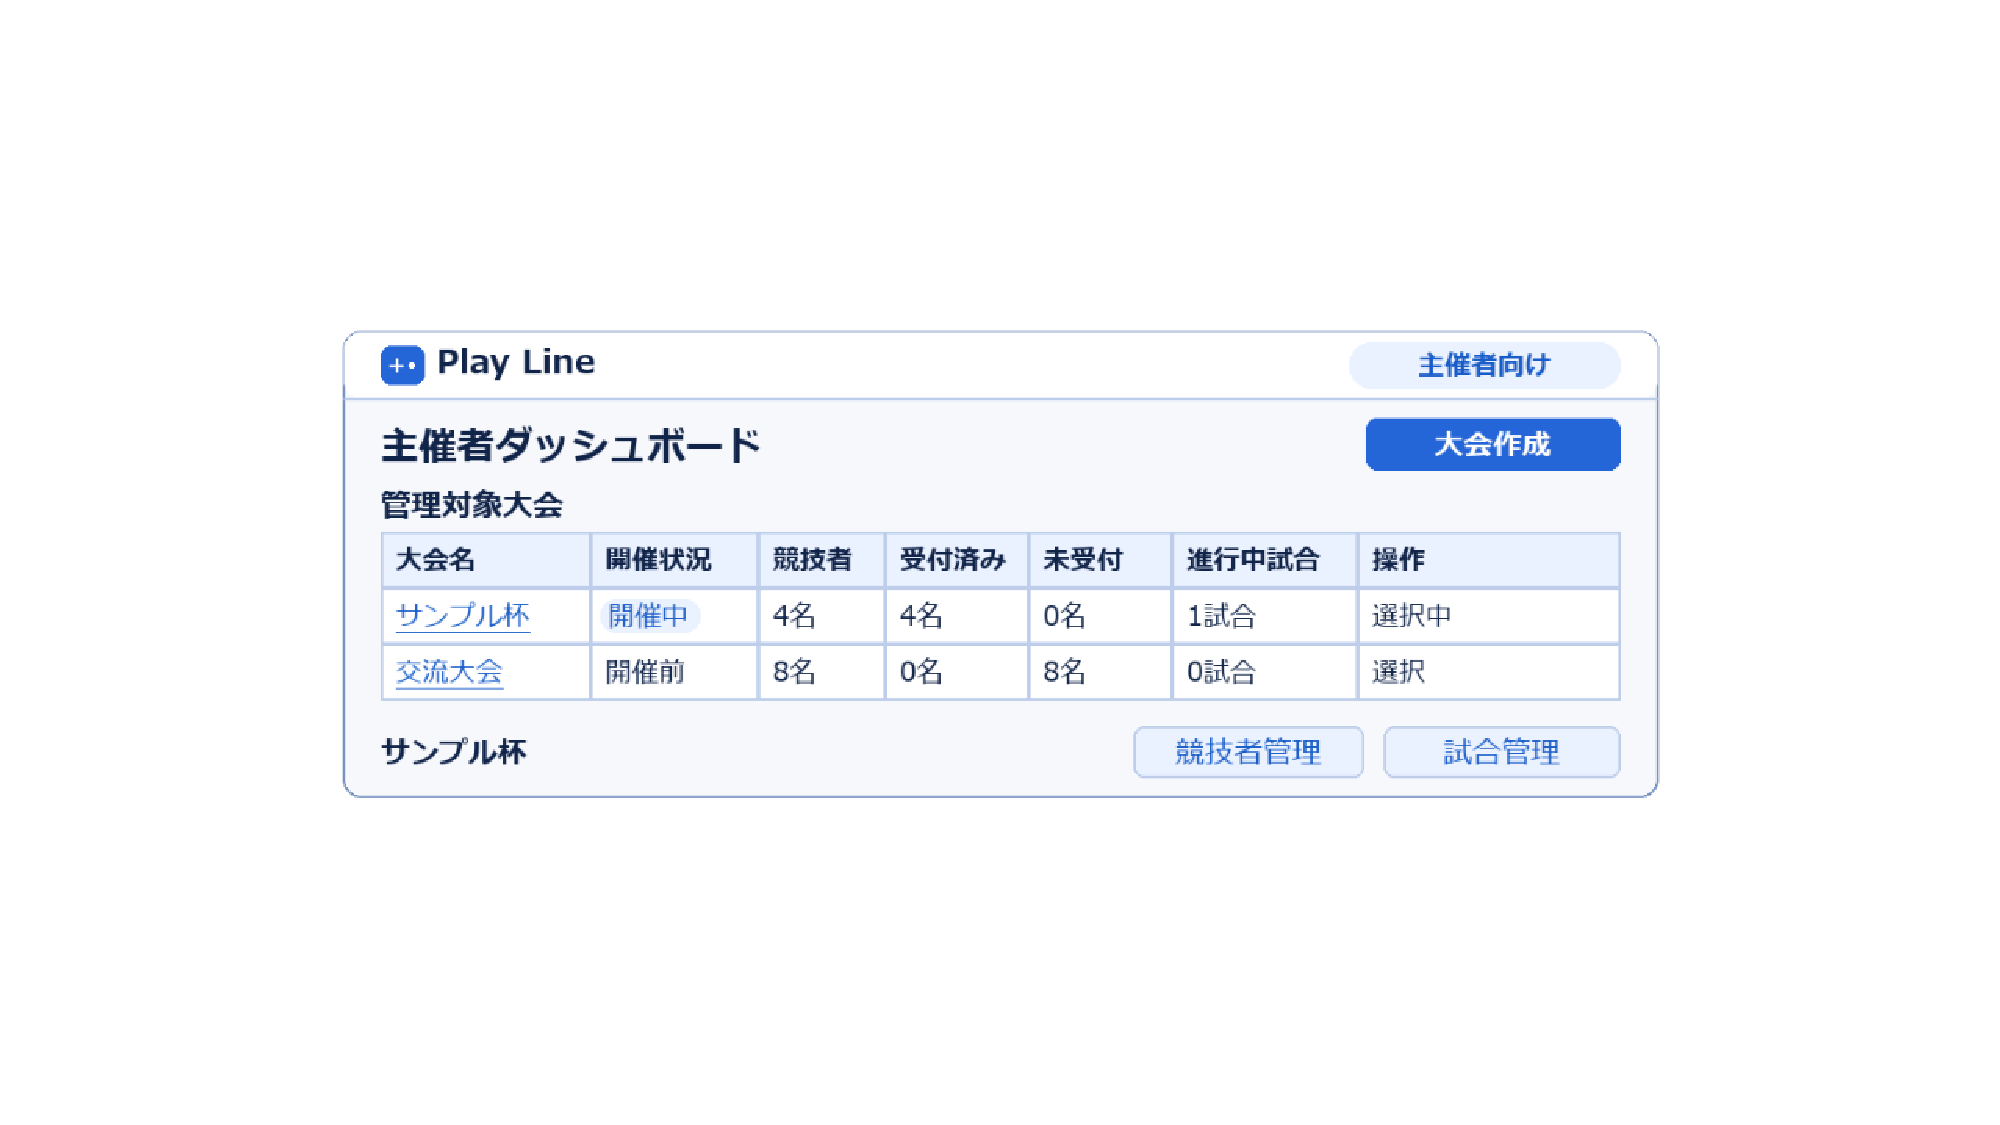
\includegraphics[width=\linewidth]{figures/04/s06_dashboard.pdf}
    \caption{主催者ダッシュボード画面 UIイメージ}
    \label{fig:ui_s06_img}
\end{figure}

\subsubsection{大会作成・編集画面（S-07）}
\begin{table}[H]
    \centering
    \caption{大会作成・編集画面のレイアウト構成}
    \label{tab:ui_s07}
    \begin{tabularx}{0.8\linewidth}{|l|X|}
        \hline
        \rowcolor{tableblue}
        \multicolumn{1}{|c|}{領域} & \multicolumn{1}{c|}{表示・入力項目} \\ \hline
        大会基本情報 & 大会名、対象ゲーム、開催日時、開催場所 \\ \hline
        参加条件 & 最大参加人数、参加受付期間、参加条件 \\ \hline
        大会設定 & シングルエリミネーション/総当たり、ルール \\ \hline
        配信設定 & ライブ配信URL \\ \hline
        操作 & 保存、公開、編集 \\ \hline
    \end{tabularx}
\end{table}

\begin{figure}[H]
    \centering
    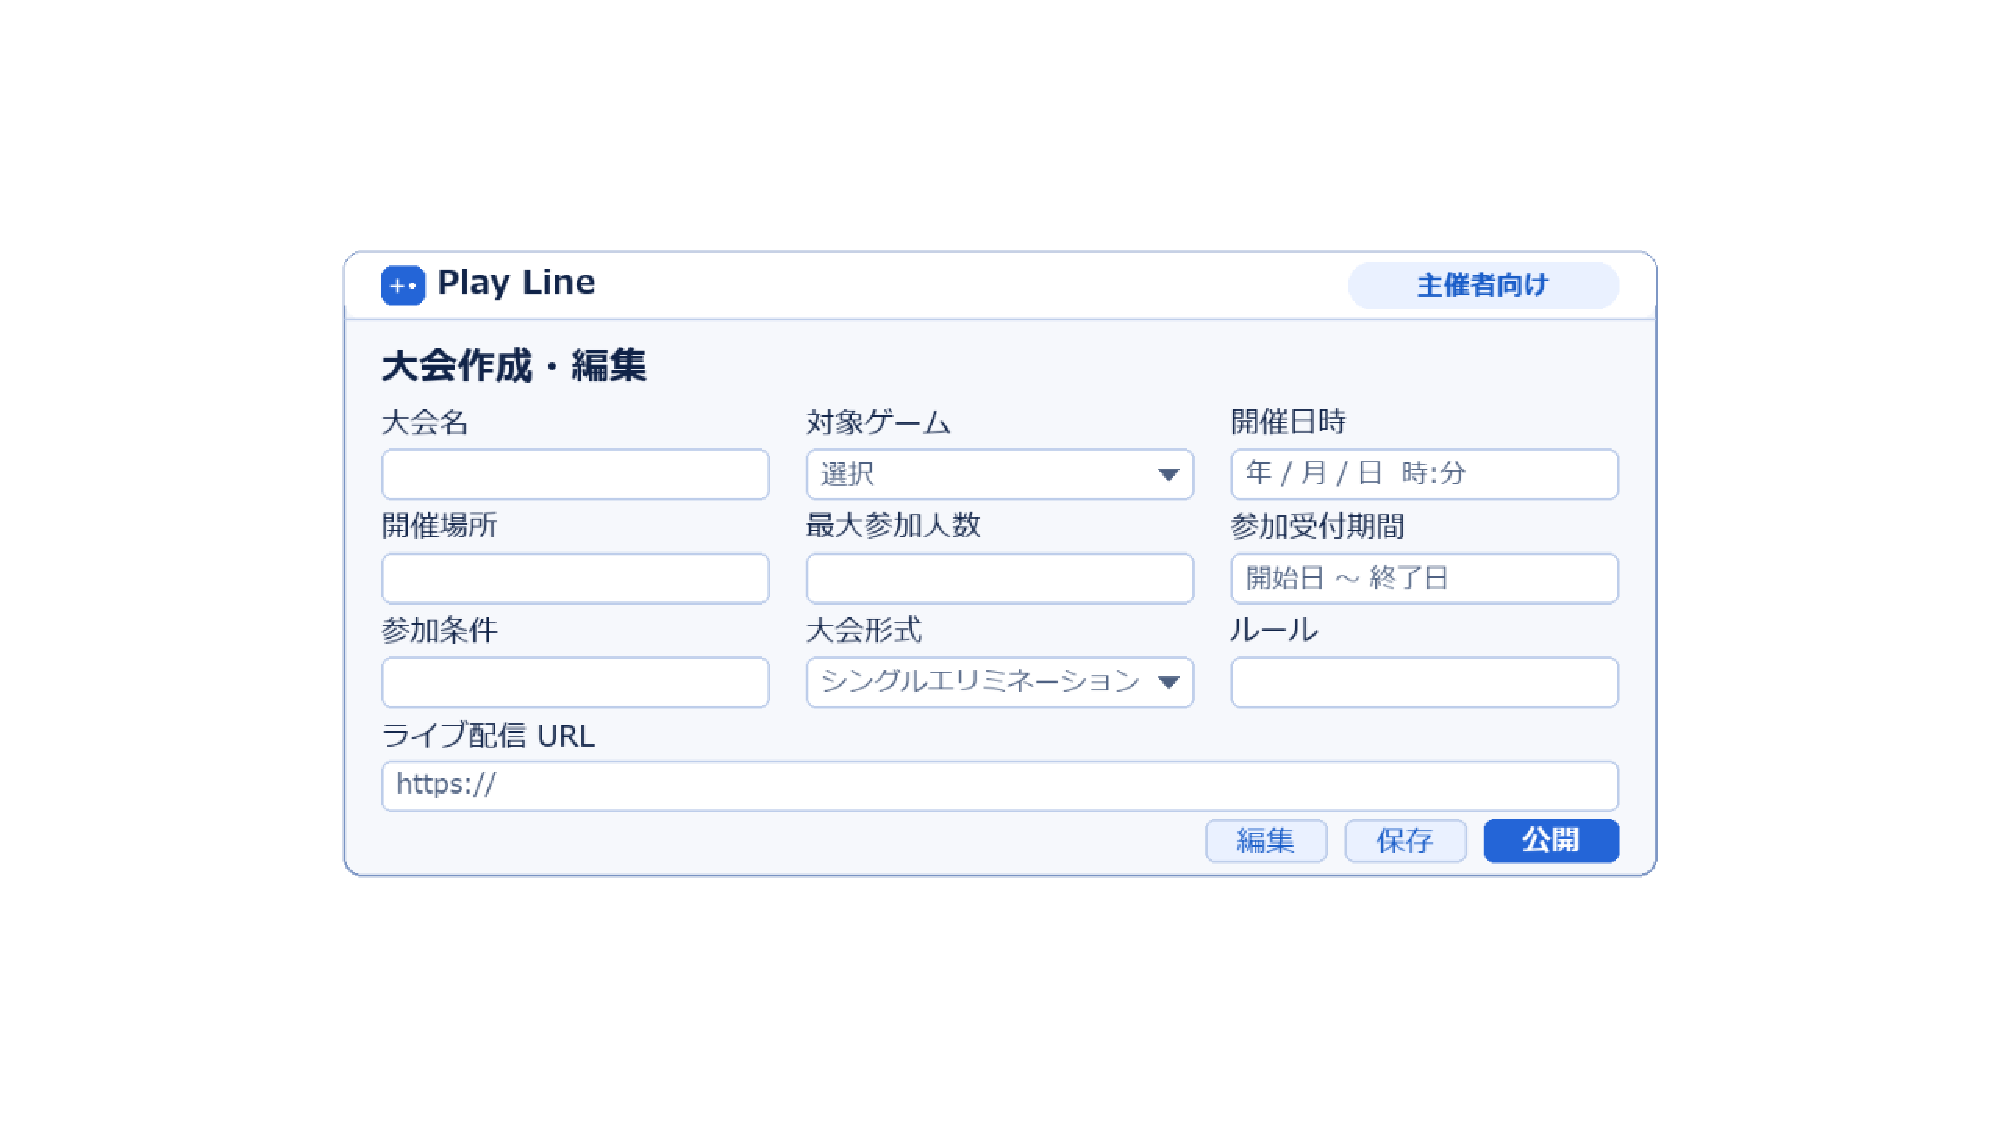
\includegraphics[width=\linewidth]{figures/04/s07_edit.pdf}
    \caption{大会作成・編集画面 UIイメージ}
    \label{fig:ui_s07_img}
\end{figure}

\subsubsection{競技者管理画面（S-08）}
\begin{table}[H]
    \centering
    \caption{競技者管理画面のレイアウト構成}
    \label{tab:ui_s08}
    \begin{tabularx}{0.8\linewidth}{|l|X|}
        \hline
        \rowcolor{tableblue}
        \multicolumn{1}{|c|}{領域} & \multicolumn{1}{c|}{表示・入力項目} \\ \hline
        検索 & 競技者名、登録状況 \\ \hline
        競技者一覧 & 氏名、プレイヤー名、参加登録状況、受付状況 \\ \hline
        操作 & 受付済み/未受付の変更、競技者情報の確認 \\ \hline
    \end{tabularx}
\end{table}

\begin{figure}[H]
    \centering
    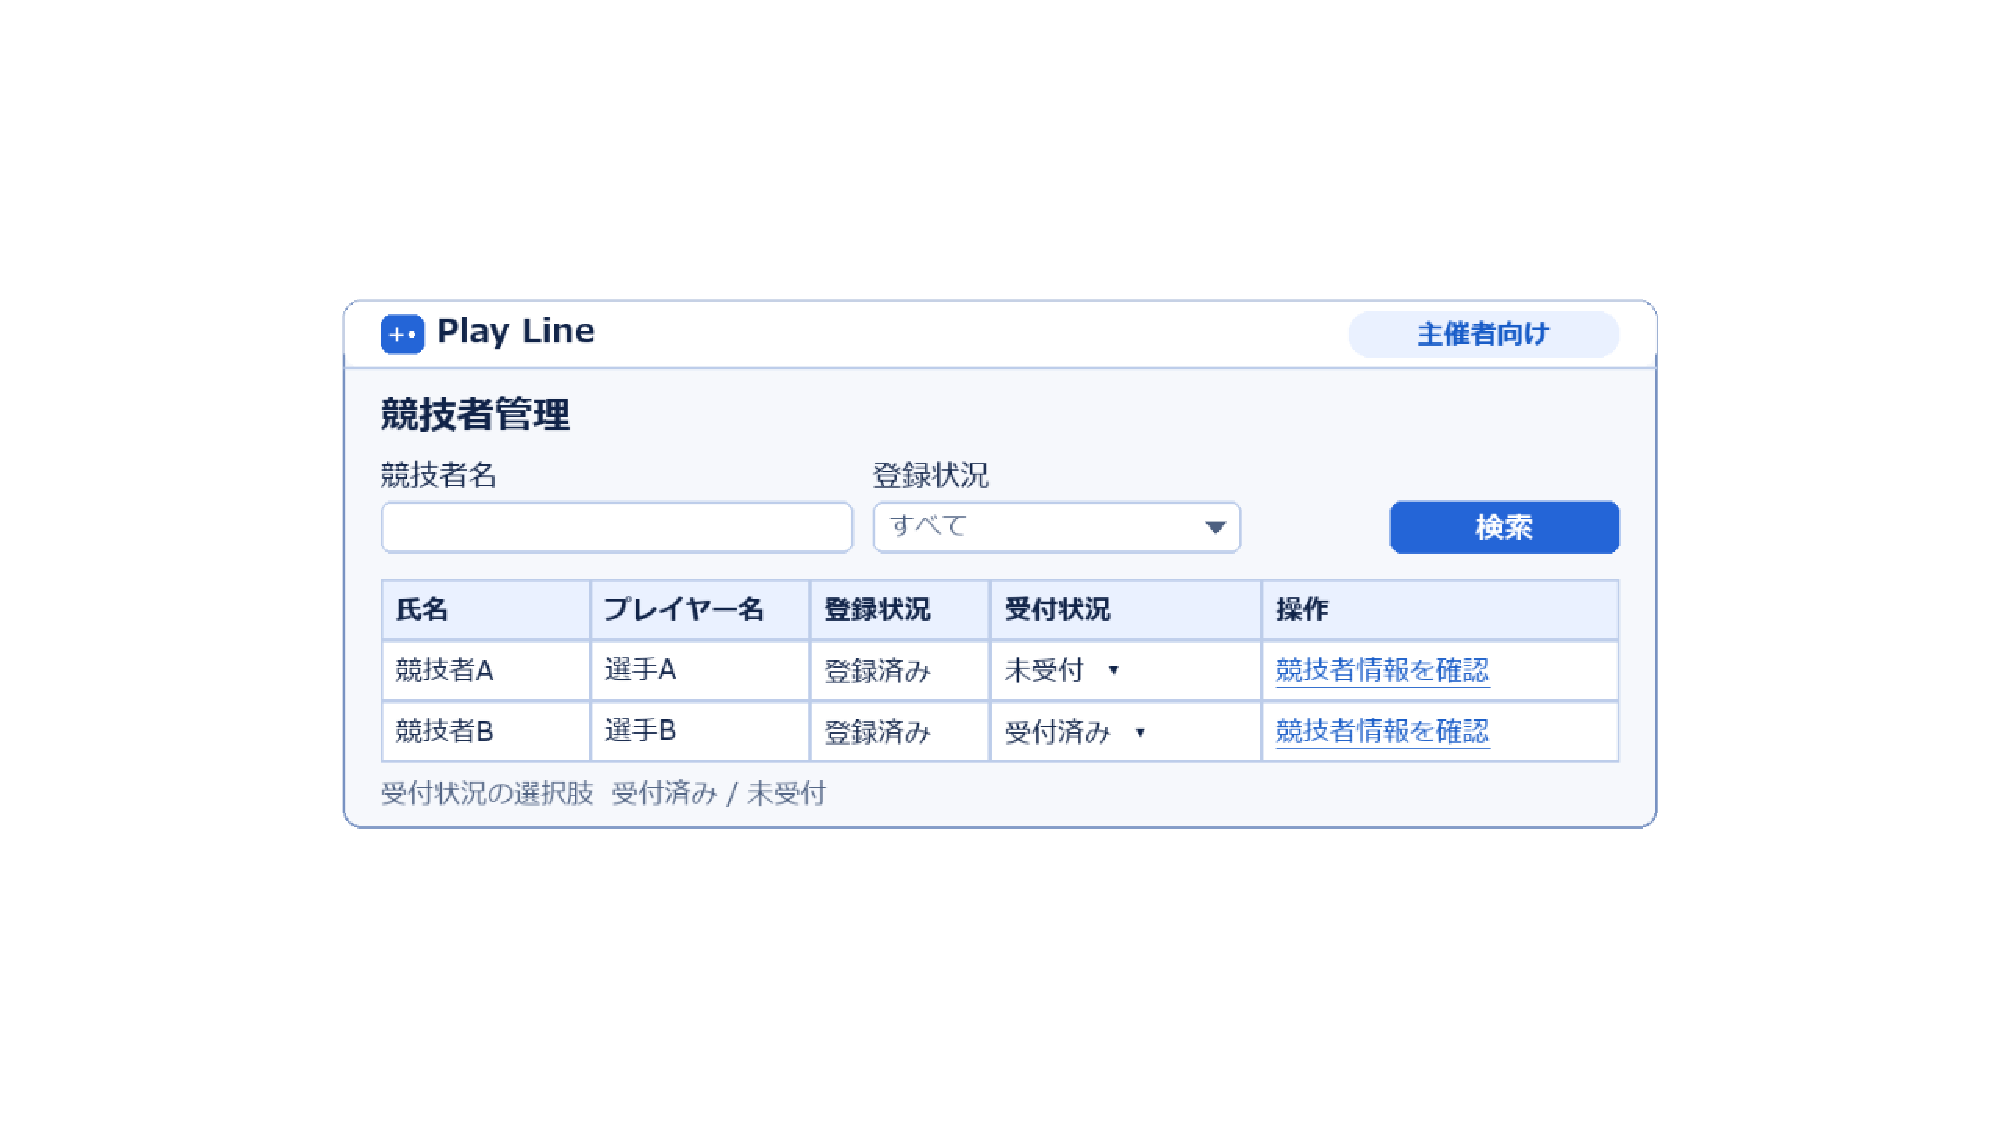
\includegraphics[width=\linewidth]{figures/04/s08_manage.pdf}
    \caption{競技者管理画面 UIイメージ}
    \label{fig:ui_s08_img}
\end{figure}

\subsubsection{トーナメント・試合管理画面（S-09）}
\begin{table}[H]
    \centering
    \caption{トーナメント・試合管理画面のレイアウト構成}
    \label{tab:ui_s09}
    \begin{tabularx}{0.8\linewidth}{|l|X|}
        \hline
        \rowcolor{tableblue}
        \multicolumn{1}{|c|}{領域} & \multicolumn{1}{c|}{表示・入力項目} \\ \hline
        トーナメント & 大会形式、対戦組み合わせ、ラウンド、試合番号 \\ \hline
        試合一覧 & 対戦者、試合状態、試合結果 \\ \hline
        結果管理 & 競技者が入力した試合結果、対戦相手の確認状態、主催者による結果の修正・登録 \\ \hline
        操作 & トーナメント作成、結果確定、結果修正、進行状況更新 \\ \hline
    \end{tabularx}
\end{table}

\begin{figure}[H]
    \centering
    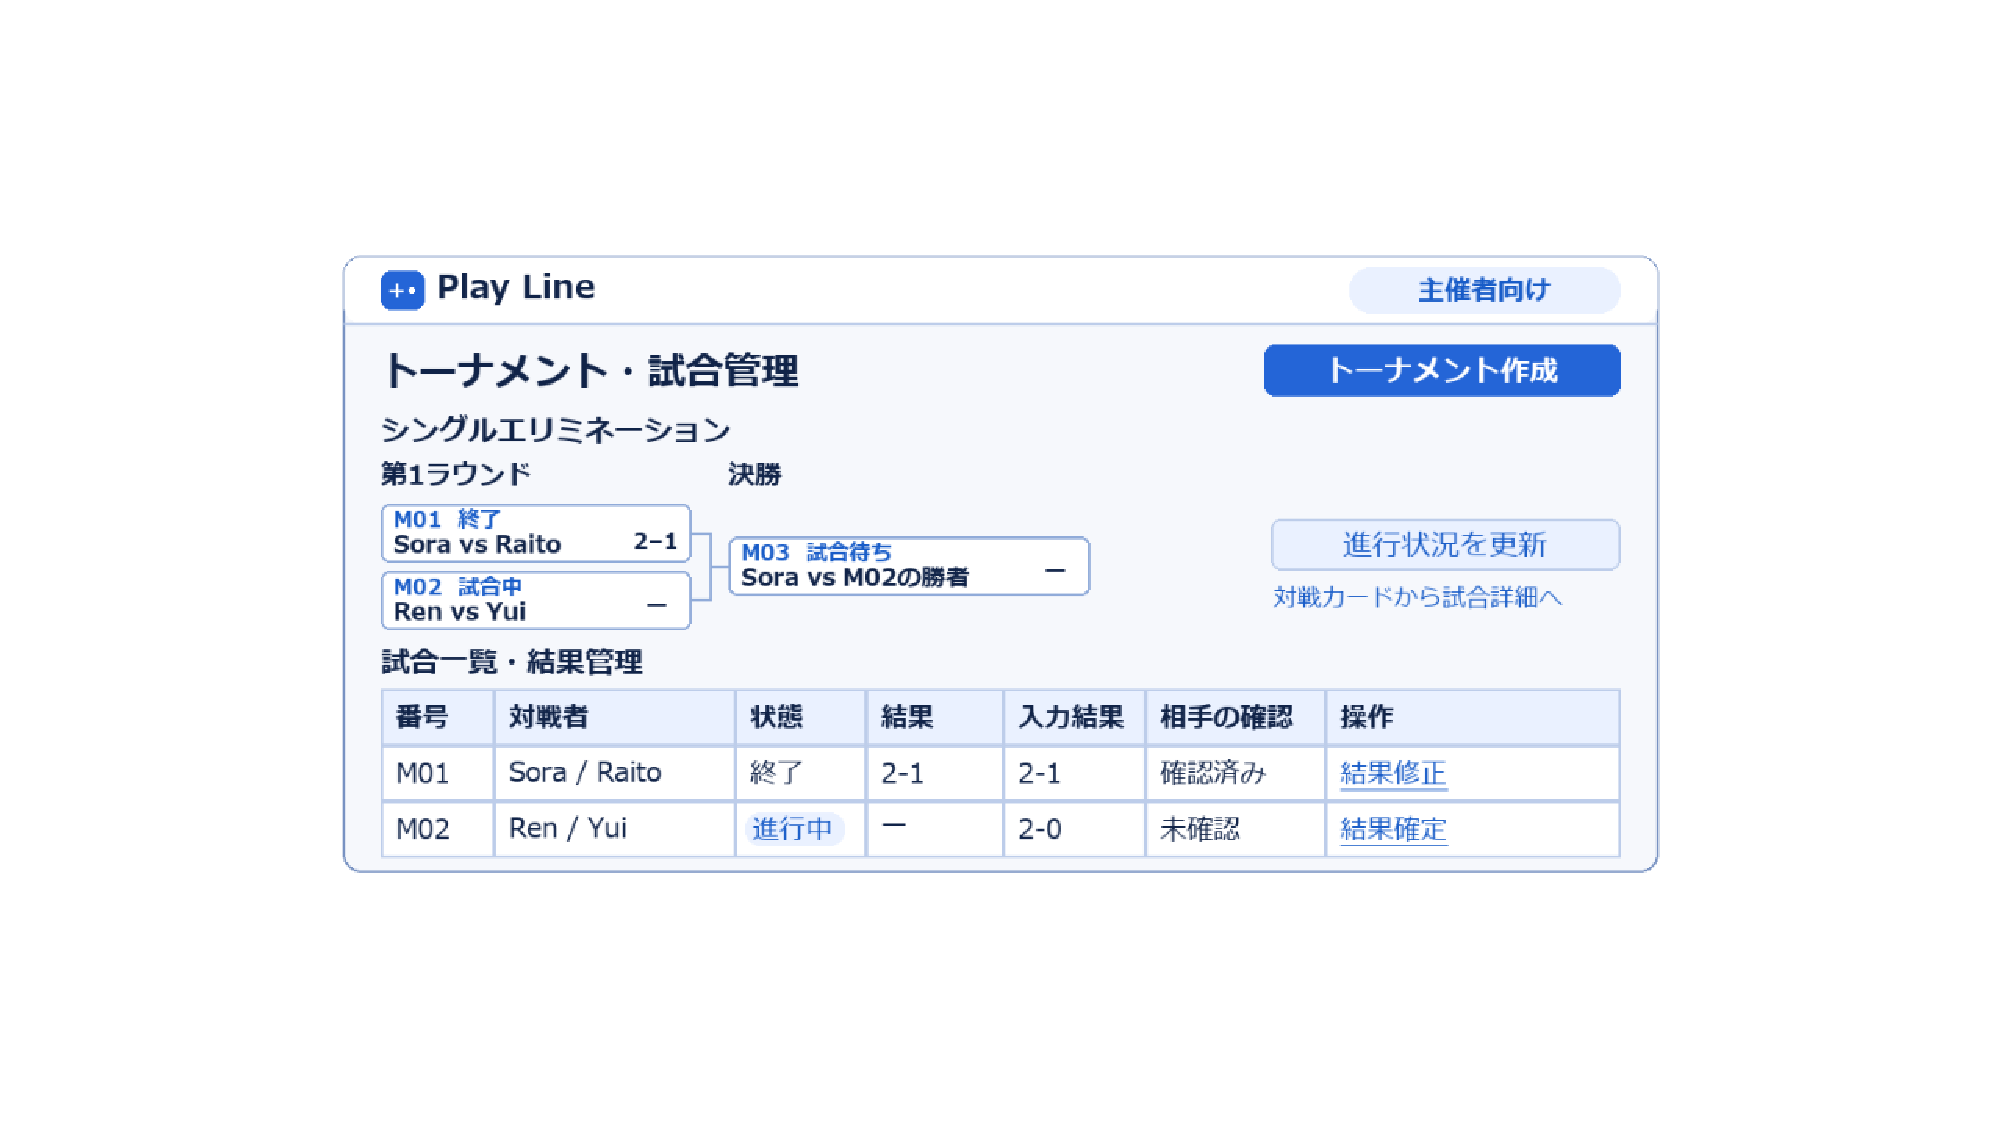
\includegraphics[width=\linewidth]{figures/04/s09_bracket.pdf}
    \caption{トーナメント・試合管理画面 UIイメージ}
    \label{fig:ui_s09_img}
\end{figure}

\subsubsection{大会観戦画面（S-10）}
\begin{table}[H]
    \centering
    \caption{大会観戦画面のレイアウト構成}
    \label{tab:ui_s10}
    \begin{tabularx}{0.8\linewidth}{|l|X|}
        \hline
        \rowcolor{tableblue}
        \multicolumn{1}{|c|}{領域} & \multicolumn{1}{c|}{表示・入力項目} \\ \hline
        大会概要 & 大会名、対象ゲーム、開催状況 \\ \hline
        大会進行 & トーナメント表、試合中・試合待ち・試合終了の一覧 \\ \hline
        注目選手 & 主催者が設定した注目選手への導線、お気に入り選手情報 \\ \hline
        配信 & ライブ配信URLへのリンク \\ \hline
    \end{tabularx}
\end{table}

\begin{figure}[H]
    \centering
    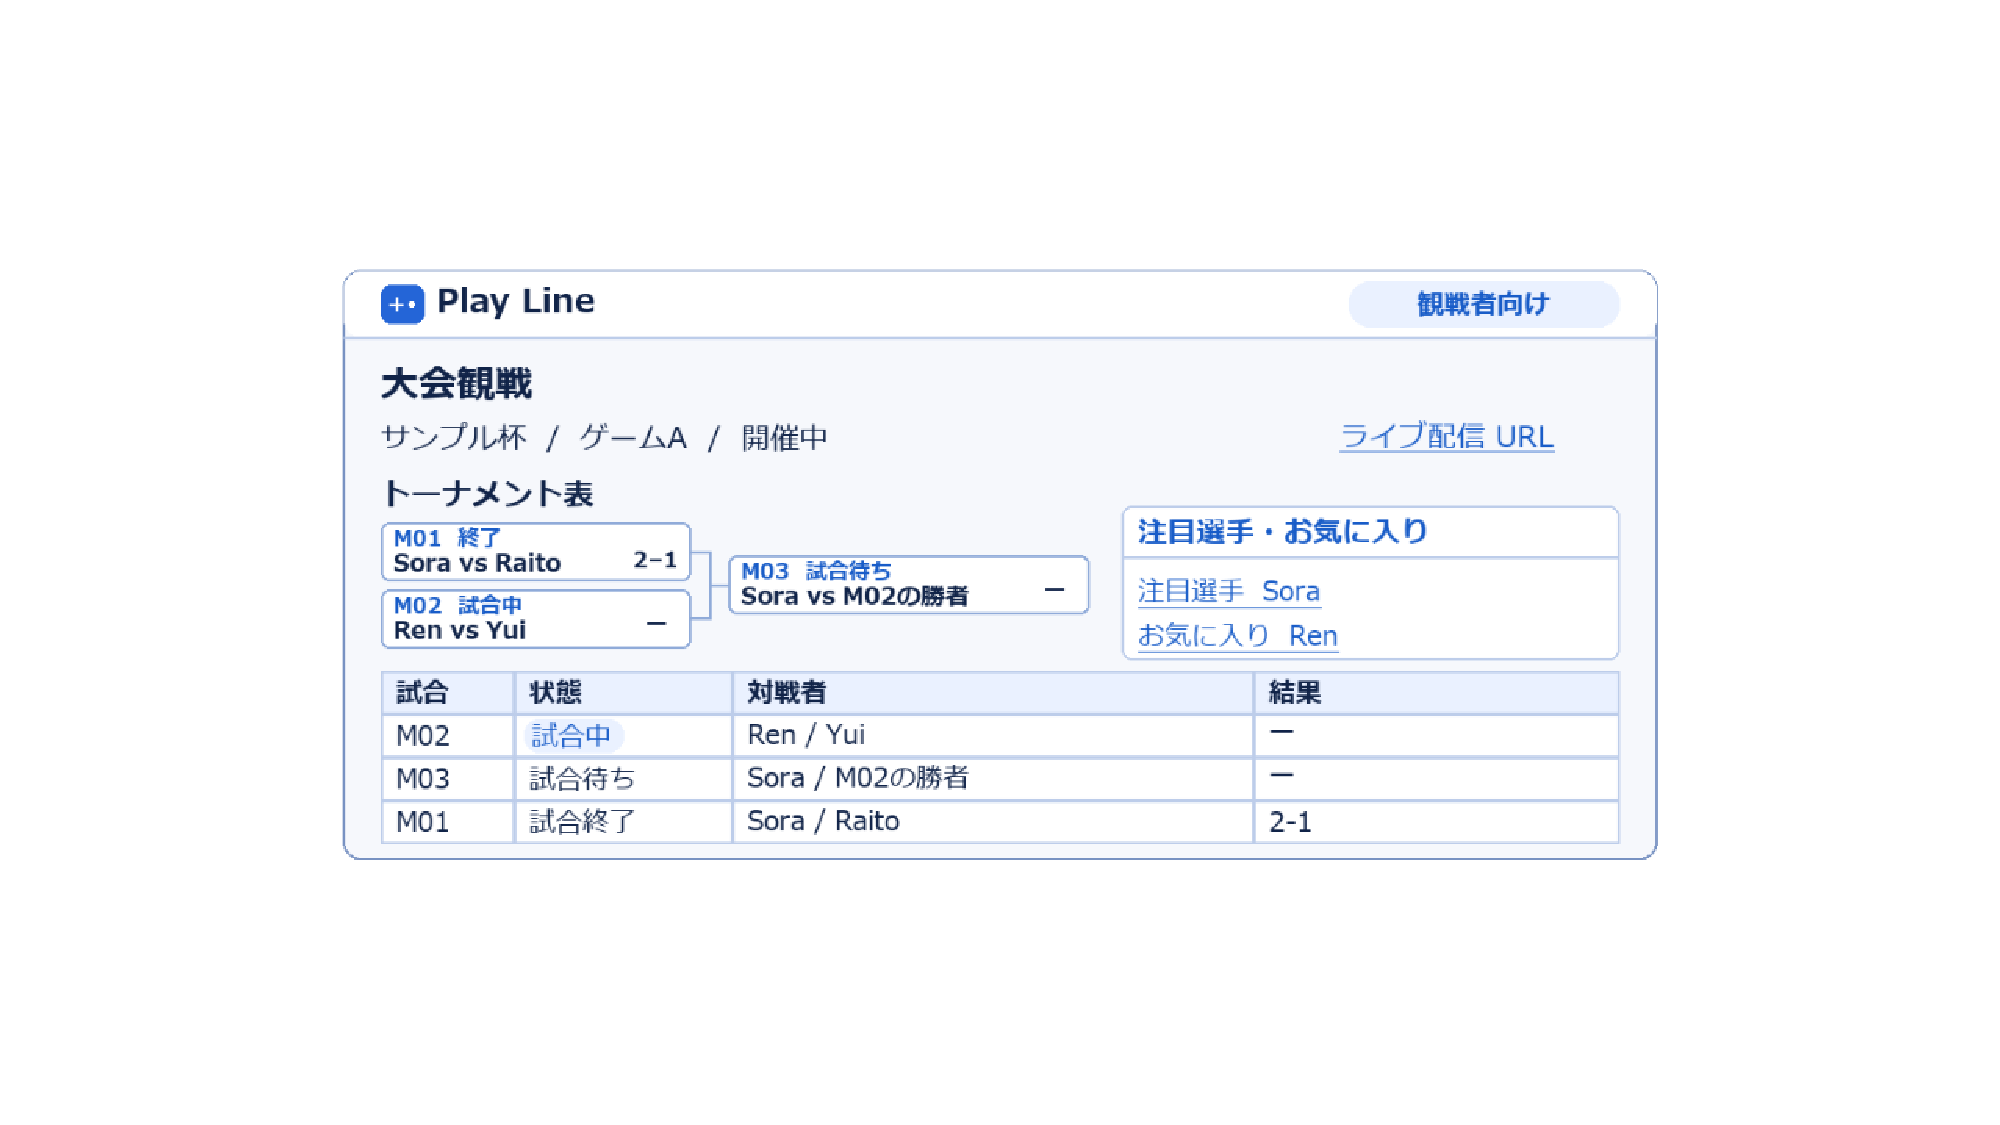
\includegraphics[width=\linewidth]{figures/04/s10_spectate.pdf}
    \caption{大会観戦画面 UIイメージ}
    \label{fig:ui_s10_img}
\end{figure}

\subsubsection{選手詳細・追跡画面（S-11）}
\begin{table}[H]
    \centering
    \caption{選手詳細・追跡画面のレイアウト構成}
    \label{tab:ui_s11}
    \begin{tabularx}{0.8\linewidth}{|l|X|}
        \hline
        \rowcolor{tableblue}
        \multicolumn{1}{|c|}{領域} & \multicolumn{1}{c|}{表示・入力項目} \\ \hline
        選手情報 & プレイヤー名、競技者を識別する固定IDに関連付けられた情報 \\ \hline
        現在の状況 & 参加大会、現在の試合、試合結果 \\ \hline
        次回試合 & 次の対戦相手、試合予定、トーナメント上の位置 \\ \hline
        過去情報 & 大会参加履歴、順位、過去の試合結果、対戦履歴 \\ \hline
        操作 & お気に入り登録 \\ \hline
    \end{tabularx}
\end{table}

\begin{figure}[H]
    \centering
    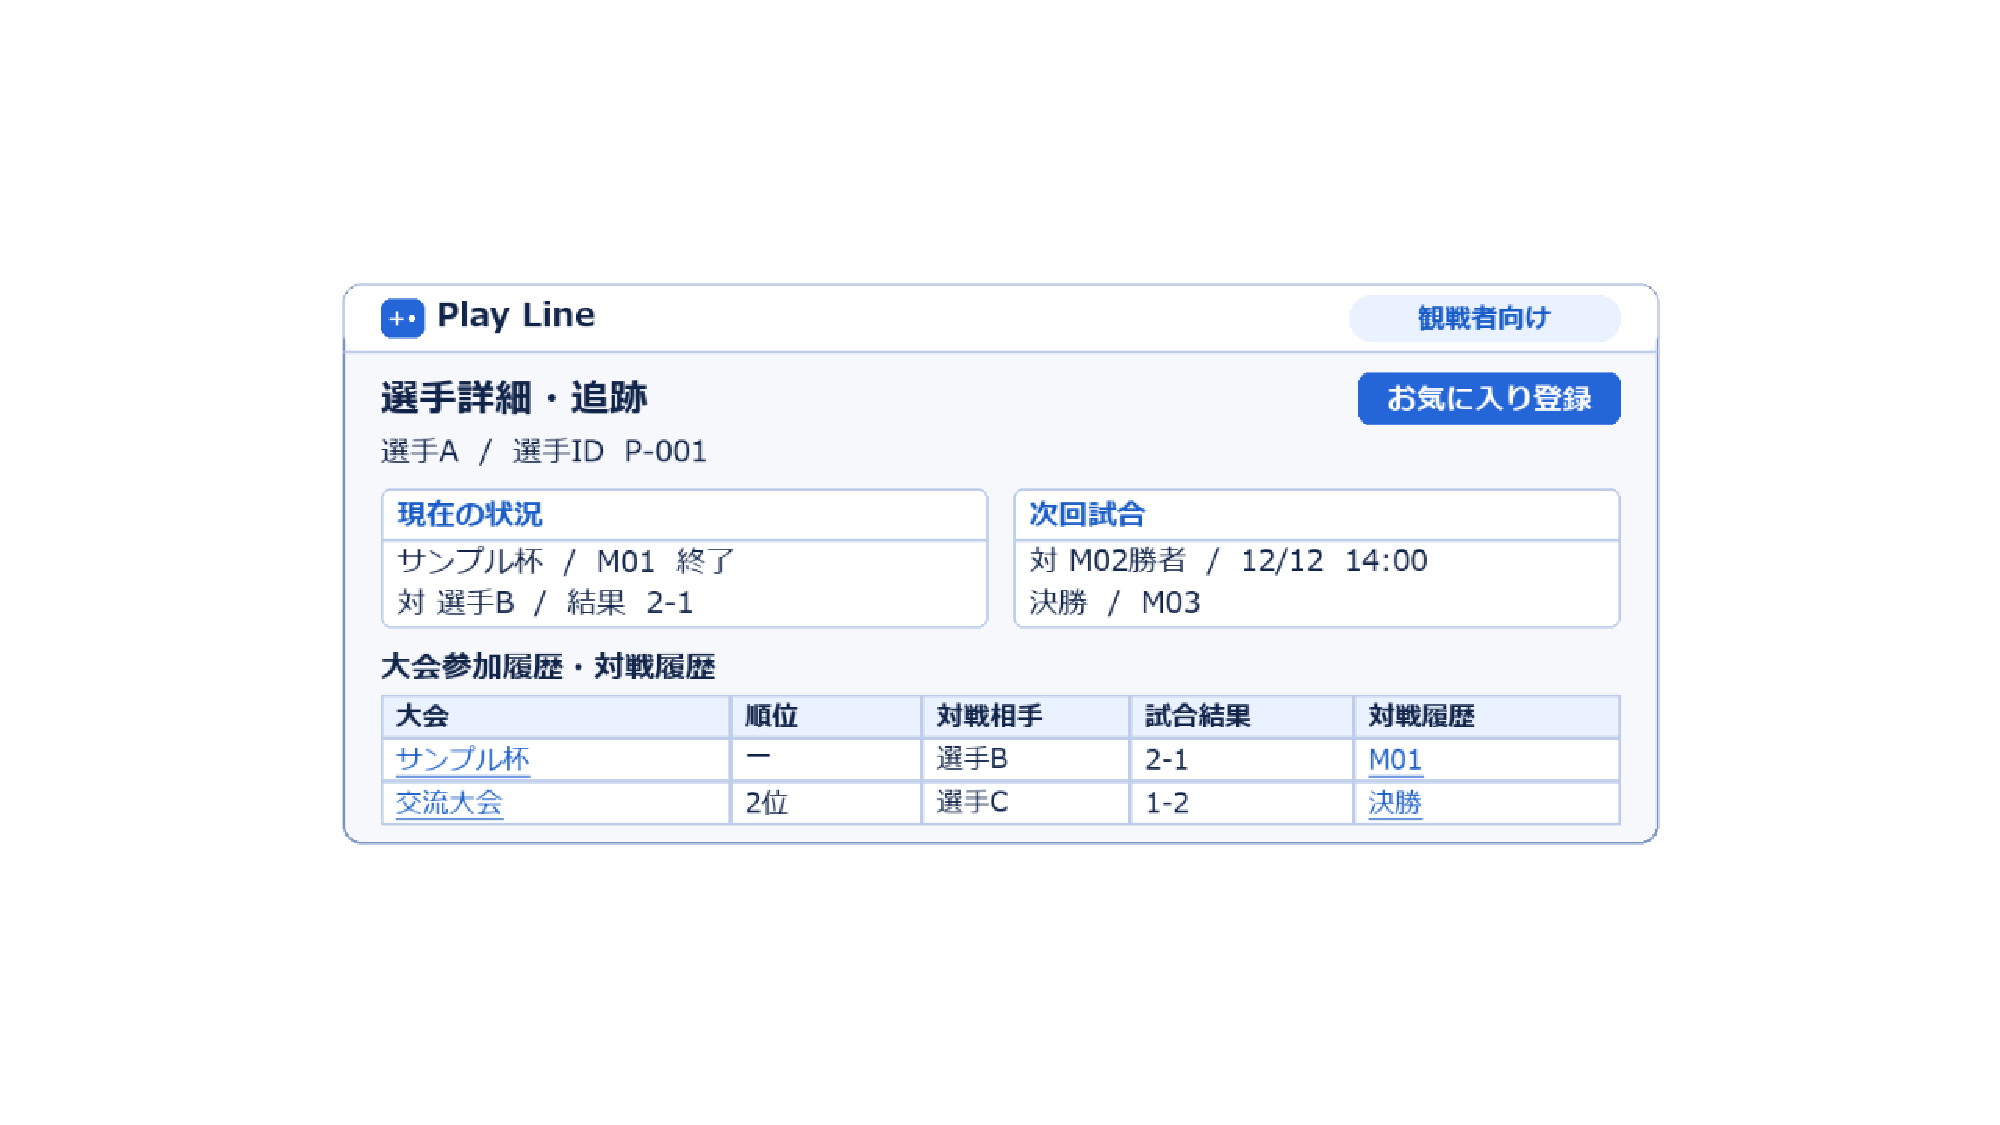
\includegraphics[width=\linewidth]{figures/04/s11_tracking.pdf}
    \caption{選手詳細・追跡画面 UIイメージ}
    \label{fig:ui_s11_img}
\end{figure}

\subsection{画面遷移}
本システムの画面間の主要な遷移関係を表\ref{tab:screen_transition}に示す。

\begin{table}[H]
    \centering
    \caption{画面遷移一覧表}
    \label{tab:screen_transition}
    \begin{tabularx}{\linewidth}{|l|l|X|}
        \hline
        \rowcolor{tableblue}
        \multicolumn{1}{|c|}{遷移元} & \multicolumn{1}{c|}{操作} & \multicolumn{1}{c|}{遷移先} \\ \hline
        S-01 ログイン & 認証成功 & 利用者の権限に応じたトップ画面 \\ \hline
        S-02 大会一覧 & 大会を選択 & S-03 大会詳細 \\ \hline
        S-03 大会詳細 & 参加登録 & S-04 競技者登録（未登録時）または参加登録処理 \\ \hline
        S-05 マイページ & 大会・試合を選択 & S-03 大会詳細、または競技者向け試合情報 \\ \hline
        S-06 ダッシュボード & 管理する大会を選択 & S-07 大会作成・編集、S-08 競技者管理、S-09 トーナメント・試合管理 \\ \hline
        S-10 大会観戦 & 選手を選択 & S-11 選手詳細 \\ \hline
        S-11 選手詳細 & 大会・試合を選択 & S-10 大会観戦 \\ \hline
    \end{tabularx}
\end{table}

\subsection{画面イメージ}
主要な画面のモックアップを図\ref{fig:ui_mockup}に示す。

\begin{figure}[H]
    \centering
    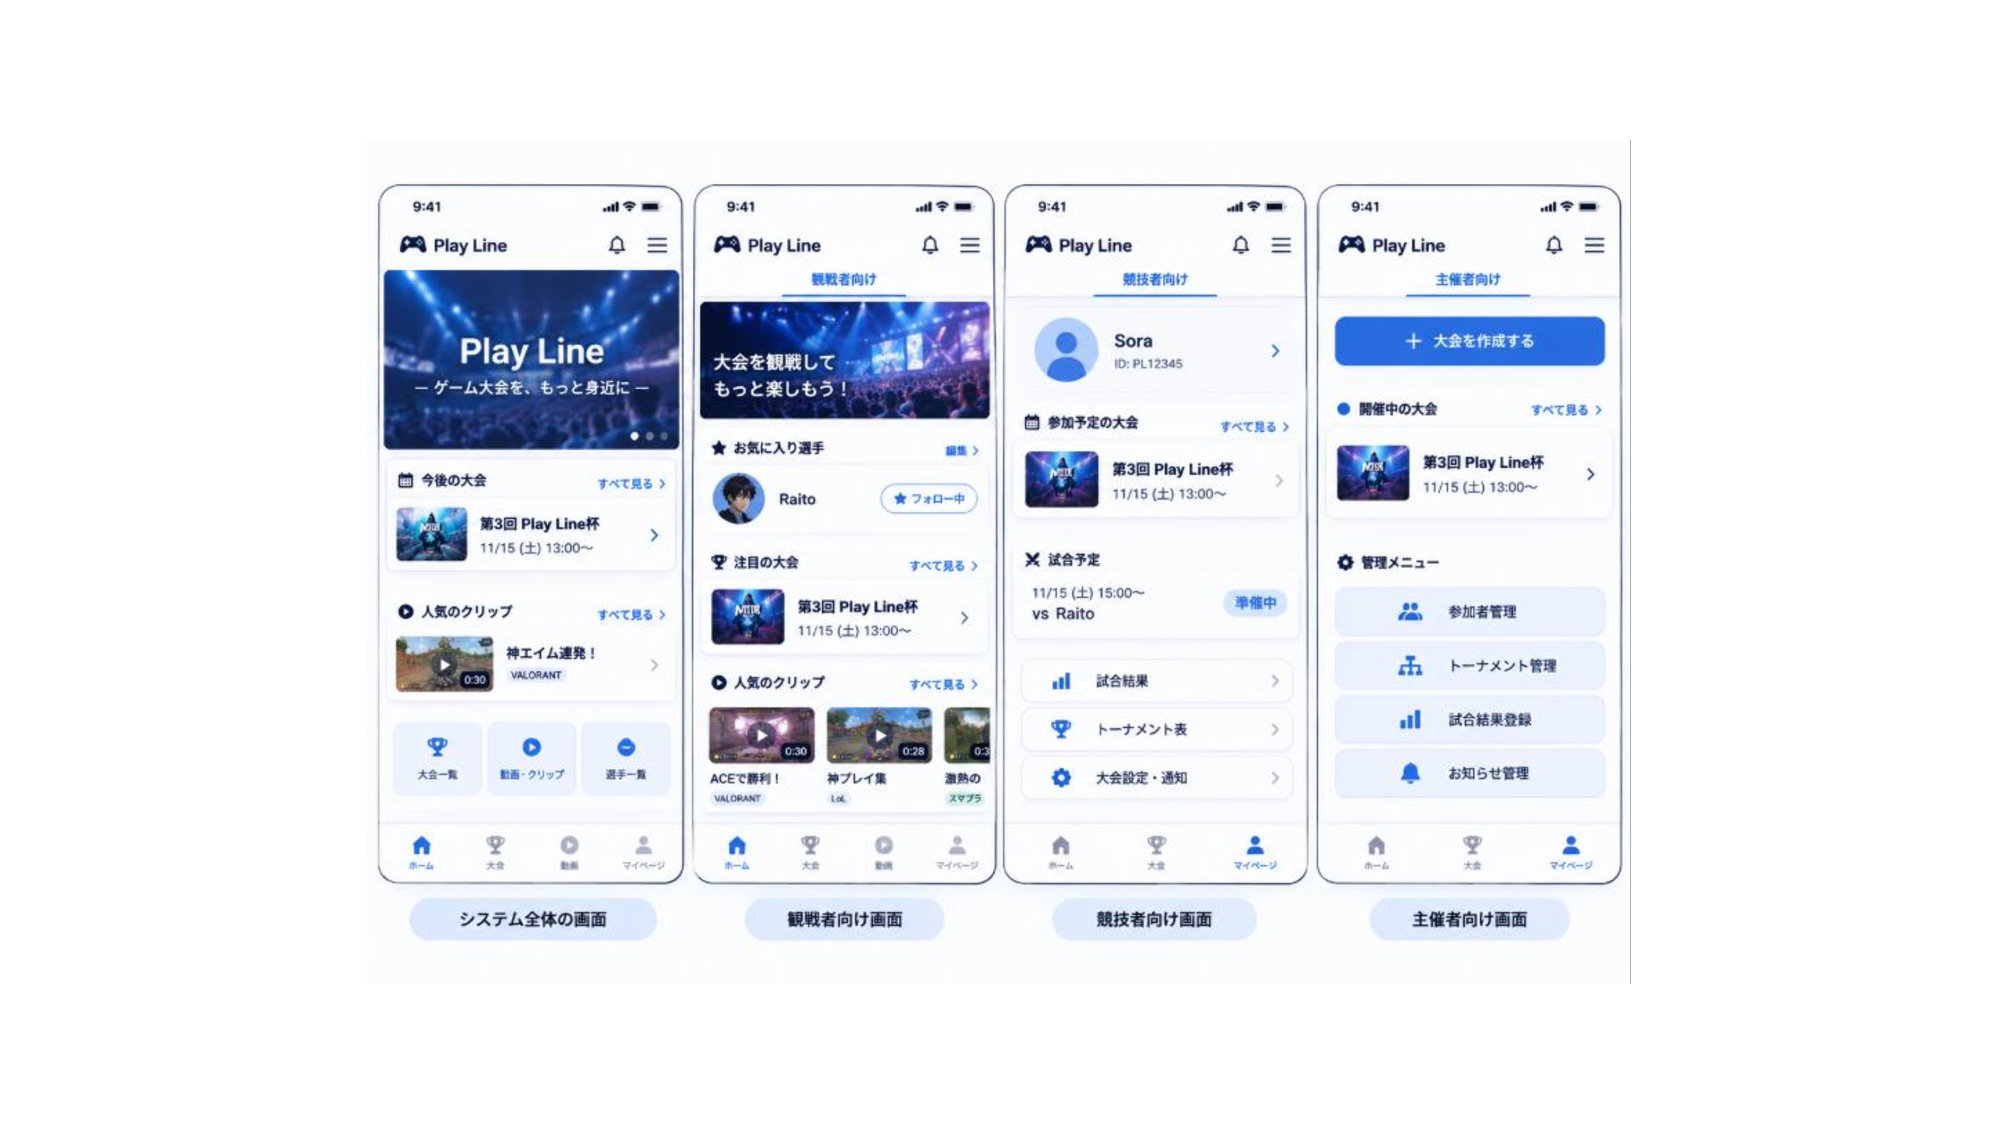
\includegraphics[width=\linewidth]{figures/04/ui_mockup.pdf}
    \caption{主要画面のレイアウト・UIイメージ}
    \label{fig:ui_mockup}
\end{figure}